\documentclass{article}
\usepackage{iclr2026_conference,times}

\input{math_commands.tex}

\usepackage{amsmath}
\usepackage{amssymb}
\usepackage{booktabs}
\usepackage{graphicx}
\usepackage{array}
\usepackage[hidelinks]{hyperref}
\usepackage{url}

\graphicspath{{../../results/figures/}}

\title{Low Energy Is Not Enough:\\Tail Audits for Energy-Based Robot Policies}

% Anonymous review mode: keep \iclrfinalcopy commented.
\author{Anonymous Authors}

\newcommand{\energy}{E_\theta}
\newcommand{\score}{S_\theta}
\newcommand{\utility}{U}
\newcommand{\candidates}{\mathcal{A}}

% \iclrfinalcopy

\begin{document}
\maketitle

\begin{abstract}
Energy-based robot policies make inference an optimization problem: sample or refine candidate actions, score them by energy, and execute the lowest-energy candidate. We show that this common selection-budget knob is selected low-energy-tail optimization rather than ordinary average-case sampling. For any fixed candidate generator, energy scorer, and utility measurement, a finite tie-aware law exactly predicts selected utility from the score groups of the candidate pool. This law makes a simple failure mode explicit: increasing \(N\) can monotonically improve selected energy while decreasing real utility if the low-energy tail is miscalibrated. We instantiate this mechanism in controlled action-selection tasks and learned IBC-style energy models, add selected-tail reliability diagrams and compute frontiers, and evaluate repair stacks that combine support penalties, pilot-label calibration, and conservative high-\(N\) gates. On supported local stress tests, the main repair stack recovers \(0.972\) of the measured oracle-minus-raw high-\(N\) gap by a predefined recovery-ratio metric. A guarded Meta-World ladder and closed-loop dependency audit provide simulator evidence while preserving the claim boundary: no real-robot validation is claimed, and autonomous learned-policy Meta-World success remains unsupported.
\end{abstract}

\section{Introduction}

Energy-based models (EBMs) are a natural fit for robot policies because they can assign low energy to multiple valid actions without averaging them into a single mean action \citep{lecun2006tutorial,florence2022implicit}. A policy for observation \(o\) defines an energy \(\energy(o,a)\) over candidate actions or short trajectories \(a\). At deployment, inference samples or refines a candidate set and executes the minimum-energy candidate. The same mechanism is used implicitly in many sampling-based policies: increasing the number of candidates is the easiest way to spend more inference compute.

The risk is that high-\(N\) inference does not test a typical model prediction. It tests the extreme low-energy tail of the learned surface. If that tail contains invalid shortcuts, out-of-support actions, or contact-bad actions, then adding candidates can make the reported energy look better while the executed action becomes worse. Average energy, training loss, and global rank correlation can miss this because the executed action is selected from a small, deployment-critical tail.

This paper formalizes and audits that selected-tail effect. We use the score convention \(\score(o,a)=-\energy(o,a)\), so tail selection chooses the maximum-score, equivalently minimum-energy, candidate. For a fixed finite pool of candidate actions, scores, and measured utilities, we give the exact expected utility of the selected item for each \(N\), including tied scores. The result is an identity, not a training guarantee: it predicts what a particular generator/scorer/utility stack will execute under tail selection.

Our contribution is a paper-ready diagnostic and evidence stack for this failure mode. First, we derive the finite selection law and use it to validate selected-utility predictions. Second, we report controlled and learned IBC-style EBM artifacts where selected energy improves with \(N\) while real utility collapses. Third, we introduce selected-tail diagnostics and reliability diagrams that ask whether the low-energy tail is useful, valid, and in support. Fourth, we evaluate repair stacks under explicit deployment assumptions. Finally, we include a guarded simulator ladder: a Meta-World selected-action benchmark, a closed-loop dependency audit, and optional non-Meta-World adapter checks. The benchmark evidence is simulator-bound and artifact-scoped; it does not claim broad manipulation success.

\section{Finite Tail-Selection Law}

\subsection{Energy policy setup}

Let \(q(a\mid o)\) be the candidate generator and let \(\energy(o,a)\) be the learned energy. We write \(\score(o,a)=-\energy(o,a)\) so that inference chooses
\begin{equation}
    \hat a_N = \arg\max_{a_i \in \{a_1,\ldots,a_N\}} \score(o,a_i),
    \qquad a_i \sim q(\cdot \mid o).
\end{equation}
Real utility \(\utility(o,a)\) is measured separately. In robot tasks it may include task reward, success, contact feasibility, smoothness, support distance, or a simulator-specific rollout metric. The selected action is evaluated by \(\utility(o,\hat a_N)\), not by energy.

\subsection{Finite tie-aware law}

Fix an observation and a finite candidate pool \(\candidates=\{a_1,\ldots,a_M\}\). Each candidate has score \(S_i\), utility \(U_i\), and proposal mass \(q_i\). Let the distinct score levels be \(s_1 > s_2 > \cdots > s_K\), with tied group \(G_k=\{i:S_i=s_k\}\), group proposal mass \(W_k=\sum_{i\in G_k}q_i\), cumulative higher-or-equal mass \(C_k=\sum_{j\le k}W_j\), and group proposal-weighted utility
\begin{equation}
    \bar U_k = \frac{1}{W_k}\sum_{i\in G_k} q_i U_i .
\end{equation}
When \(N\) candidates are drawn independently from \(q\), the probability that the selected score level lies in group \(G_k\) is
\begin{equation}
    p_{k,N} = (1-C_{k-1})^N - (1-C_k)^N,
    \qquad C_0=0 .
\end{equation}
Therefore the exact selected utility is
\begin{equation}
    \mathbb{E}[\utility(\hat a_N)] =
    \sum_{k=1}^{K} p_{k,N} \bar U_k .
    \label{eq:finite-law}
\end{equation}
The uniform finite-pool case is recovered by \(q_i=1/M\). Ties are handled by the group average: conditional on the selected score level, the selected tied item has the proposal-weighted utility of that score group. Equation~\ref{eq:finite-law} is a deployment audit for a fixed generator, scorer, and utility. It implies that high-\(N\) performance depends on the utility of score levels that receive new selection mass as \(N\) grows.

\paragraph{Selected-tail implication.}
For EBMs, larger \(N\) shifts selection mass toward lower energy quantiles. Tail selection improves selected utility exactly when those lower-energy quantiles have higher utility than the mass they replace. If the low-energy tail is anti-aligned with utility, increasing \(N\) can reduce energy and utility simultaneously. This is the failure signature we audit.

\section{Diagnostics and Repairs}

We report metrics at the selected action and in the selected tail. The core selected metrics are selected energy, selected score, selected utility, success, invalid-action rate, contact failure, smoothness penalty, support distance, high-\(N\) regret, oracle gap, and marginal utility per added candidate. Tail metrics bucket the candidate pool by energy quantile and report mean real utility, success, invalid rate, contact failure, support distance, and whether the bucket is the extreme low-energy tail.

The repair ladder separates assumptions. Support penalties and conservative stopping use no utility labels. Pilot-label calibration uses a small held-out set of measured utilities to recalibrate the energy ranking. Value-shaped scoring and oracle scoring are upper-bound repairs that use more direct utility information. The main repair stack is calibrated, support-penalized scoring with a conservative high-\(N\) gate. Its metric is fixed in advance:
\begin{equation}
    \mathrm{recovery} =
    \frac{U_{\mathrm{repair}} - U_{\mathrm{raw}}}
         {U_{\mathrm{oracle}} - U_{\mathrm{raw}}}.
    \label{eq:recovery}
\end{equation}
We use near-complete repair language only when the mean recovery ratio exceeds \(0.95\), the worst supported stress case remains above the configured threshold, and utility-degrading rows are reported rather than hidden.

\section{Experiments}

\paragraph{Controlled low-energy-tail failures.}
We use two controlled action-selection settings: a contact-rich push/insert task and a multimodal obstacle task. Energy variants include oracle, aligned, raw miscalibrated, shortcut, smoothness-blind, out-of-distribution-low-energy, support-blind, noisy, and pilot-label-noise scorers. Candidate counts range from \(N=1\) to \(N=512\).

\paragraph{Learned IBC-style EBMs.}
We train a NumPy linear-feature EBM and a PyTorch MLP EBM with an InfoNCE-style contrastive objective over one expert or high-value action and negative action samples \citep{gutmann2010noise,oord2018representation,florence2022implicit}. The NumPy model is intentionally observation-limited and can learn a shortcut low-energy tail; the PyTorch model demonstrates an aligned-tail regime under the same finite-law audit.

\paragraph{Repair, reliability, and compute.}
Repair experiments compare raw, support-penalized, calibrated, value-shaped, conservative-gated, and oracle scoring. Reliability experiments bucket candidates by energy quantile. Compute-frontier experiments compare sample-only scoring, CEM-like top-\(k\) refinement, and Langevin-like refinement under energy-evaluation budgets \citep{rubinstein1999crossentropy,deboer2005tutorial}.

\paragraph{Simulator ladder.}
The Meta-World ladder covers reach-v3, push-v3, pick-place-v3, and button-press-v3 \citep{yu2020metaworld}. The primary benchmark EBM is trained on scripted expert actions; high-reward sampled positives are kept only as an ablation. Its selected-action benchmark executes the selected first action followed by scripted continuation, so it is not autonomous learned-policy evidence. A separate closed-loop dependency audit executes policies without scripted continuation and compares expert-centered, nearest-demo, behavior-cloned, state-heuristic, local Gaussian, random, and scripted variants. Optional Gymnasium, ManiSkill, and robosuite adapters are finite guarded rollout checks \citep{towers2024gymnasium,gu2023maniskill2,zhu2020robosuite}.

\section{Results}

\subsection{Finite law predicts selected utility}

Across the exact-law validation artifacts, Equation~\ref{eq:finite-law} matches Monte Carlo selected-utility estimates with mean absolute error \(0.0037\), RMSE \(0.0058\), and maximum absolute error \(0.0137\). This confirms that the later curves can be interpreted as properties of the fixed candidate/scorer/utility stacks rather than sampling noise.

\subsection{Energy can improve while utility collapses}

Figure~\ref{fig:energy-utility-drop} shows the central failure. In the strongest controlled row, a raw miscalibrated EBM on the multimodal task moves from selected energy \(-1.839\) at \(N=1\) to \(-2.988\) at \(N=512\), while selected real utility falls from \(0.341\) to \(-1.538\). The low-energy tail utility is \(-1.480\), the energy-utility rank correlation is \(-0.163\), invalid-action rate is \(1.0\), support distance is \(0.982\), and high-\(N\) regret is \(3.225\). The learned NumPy IBC artifact reproduces the same mechanism: at \(N=512\), raw selected utility is \(-1.453\), invalid rate is \(0.996\), and calibration improves high-\(N\) utility by \(3.003\). The PyTorch MLP EBM provides the contrasting aligned case, with selected utility \(1.615\), success essentially \(1.0\), and high-\(N\) regret \(0.078\).

\begin{figure}[t]
    \centering
    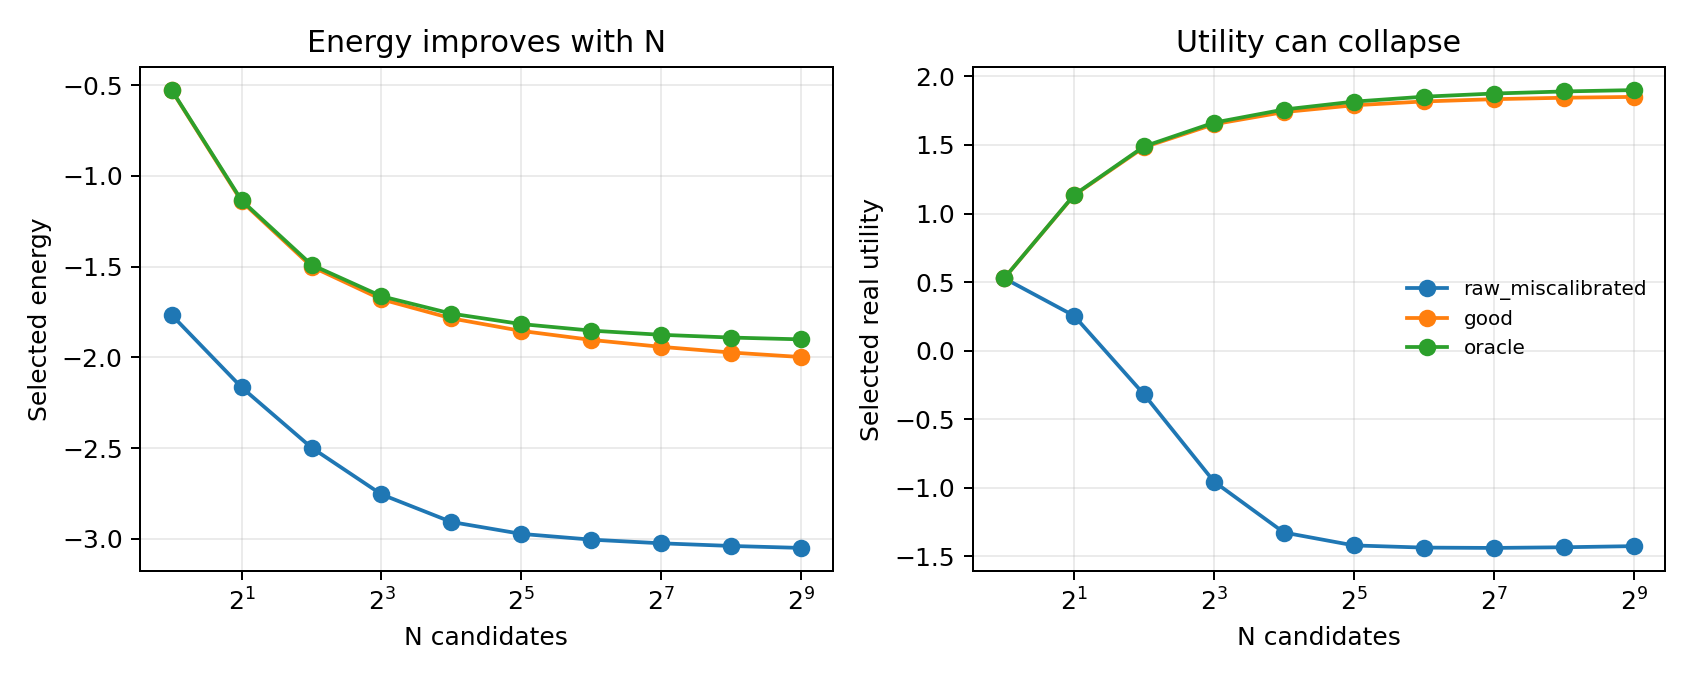
\includegraphics[width=0.95\linewidth]{figure1_energy_utility_drop.png}
    \caption{Selected energy can improve while selected real utility degrades. The failure is not that energy is high; it is that the lowest-energy tail is not the highest-utility tail.}
    \label{fig:energy-utility-drop}
\end{figure}

\subsection{Repairs help only when they repair the selected tail}

Figure~\ref{fig:repair} summarizes the repair hierarchy. On supported high-\(N\) repair stress tests at \(N=512\), the main calibrated support-penalized conservative-gate stack reaches mean recovery \(0.972\), worst-case recovery \(0.962\), recovery-at-least-\(0.95\) rate \(1.0\), and zero utility-degrading rows. It still reports one repair failure from a tail-rank-improvement diagnostic. Support-only repairs improve utility but do not satisfy the near-complete threshold: support-penalized recovery is \(0.886\), and support-penalized conservative-gate recovery is \(0.870\). This is why the claim is metric-bound rather than universal.

\begin{figure}[t]
    \centering
    \begin{minipage}{0.49\linewidth}
        \centering
        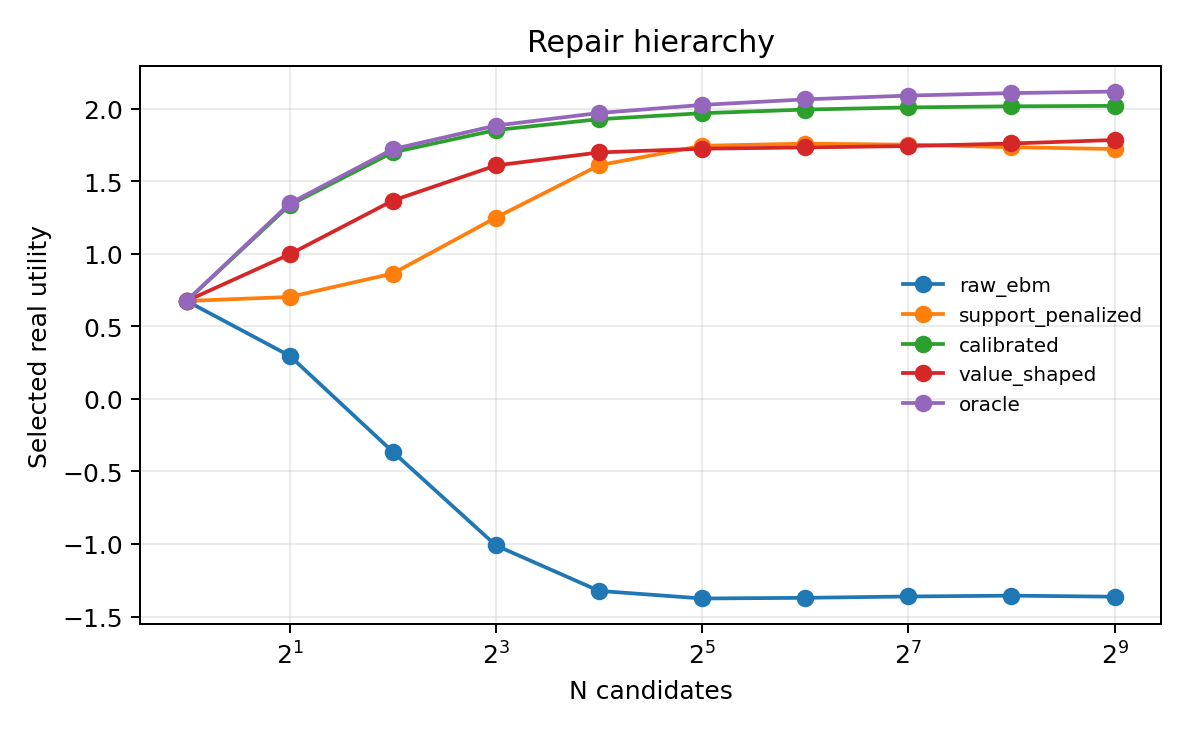
\includegraphics[width=\linewidth]{figure2_repair_comparison.png}
    \end{minipage}
    \begin{minipage}{0.49\linewidth}
        \centering
        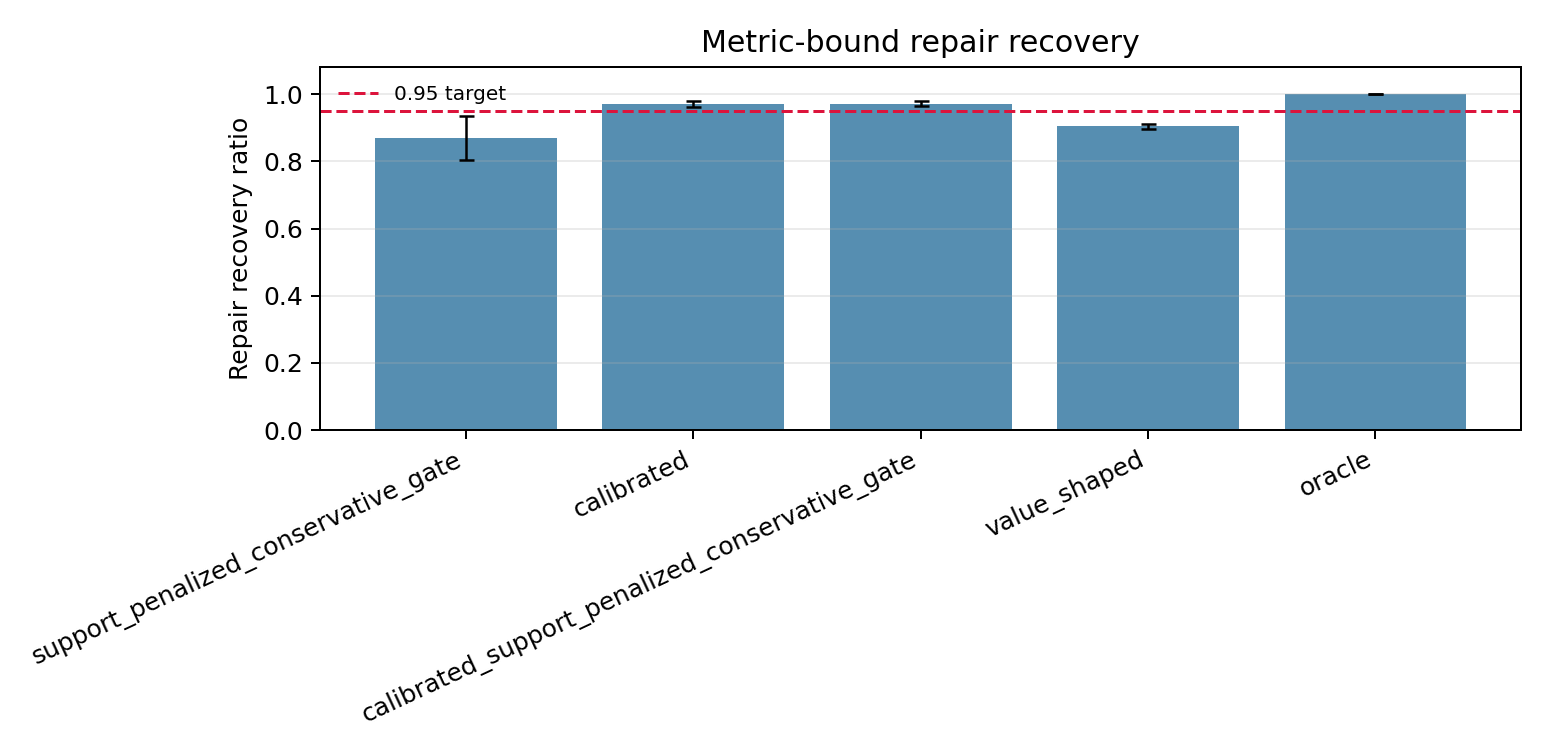
\includegraphics[width=\linewidth]{figure8_repair_recovery_ratio.png}
    \end{minipage}
    \caption{Repair comparison and recovery ratio. Near-complete repair refers only to Equation~\ref{eq:recovery} on supported local stress artifacts.}
    \label{fig:repair}
\end{figure}

\subsection{Reliability and compute frontiers expose tail risk}

Energy reliability diagrams in Figure~\ref{fig:reliability-compute} bucket candidates by energy quantile. The goal is not calibration in the usual probability sense alone \citep{guo2017calibration}; it is selected-tail reliability: do lower-energy buckets have better task utility, lower invalid rate, and lower support distance? The compute frontier shows why this matters. Additional candidates and refinement steps increase energy evaluations and can improve the objective being optimized while moving real utility in the wrong direction. Conservative stopping is therefore a deployment decision, not only an efficiency decision.

\begin{figure}[t]
    \centering
    \begin{minipage}{0.49\linewidth}
        \centering
        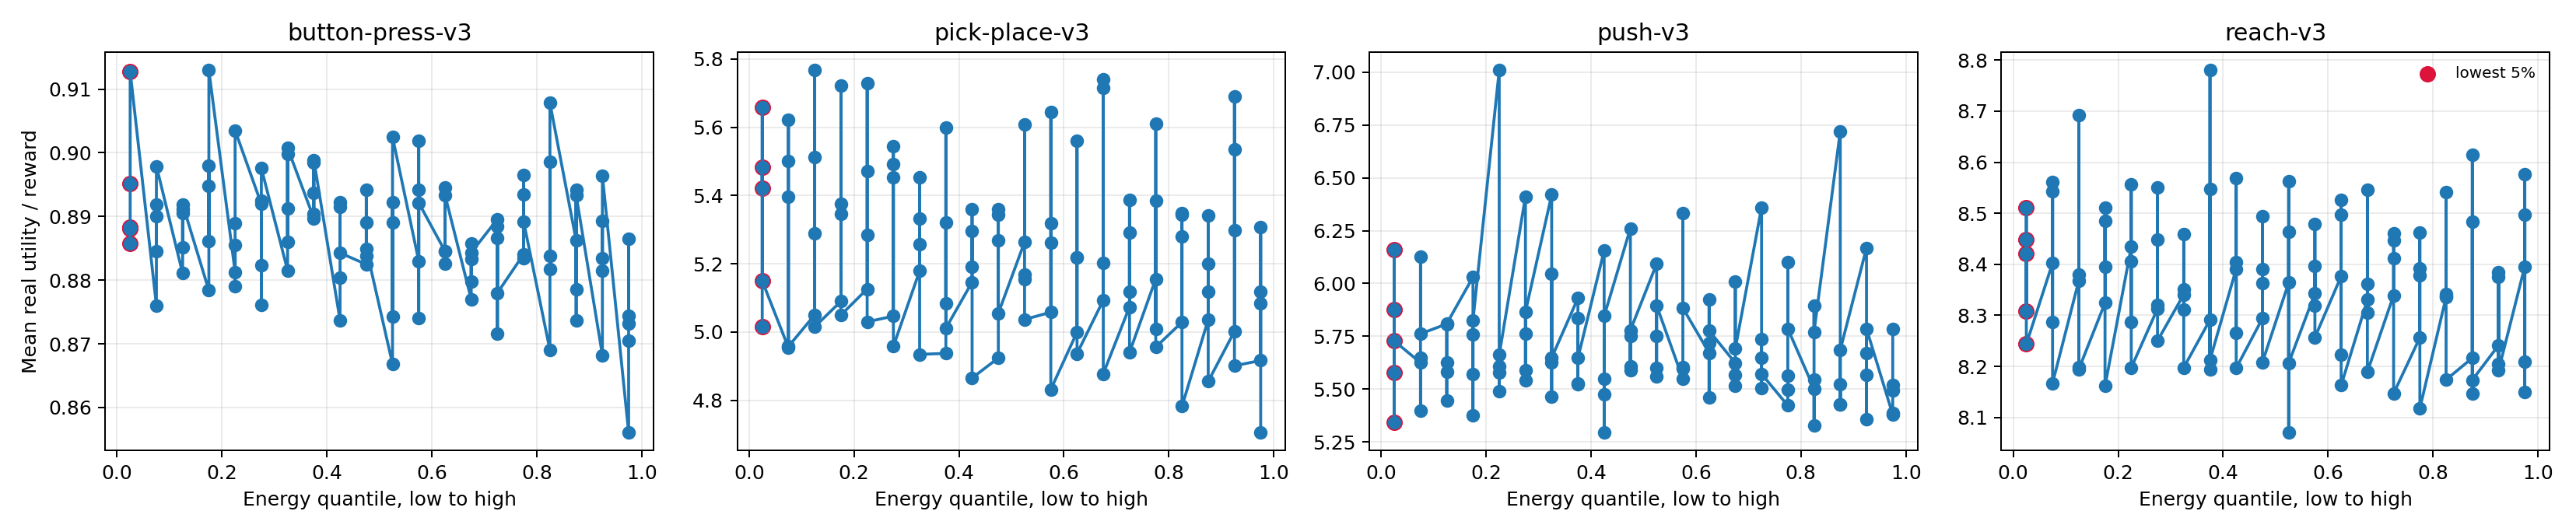
\includegraphics[width=\linewidth]{figure3_tail_reliability.png}
    \end{minipage}
    \begin{minipage}{0.49\linewidth}
        \centering
        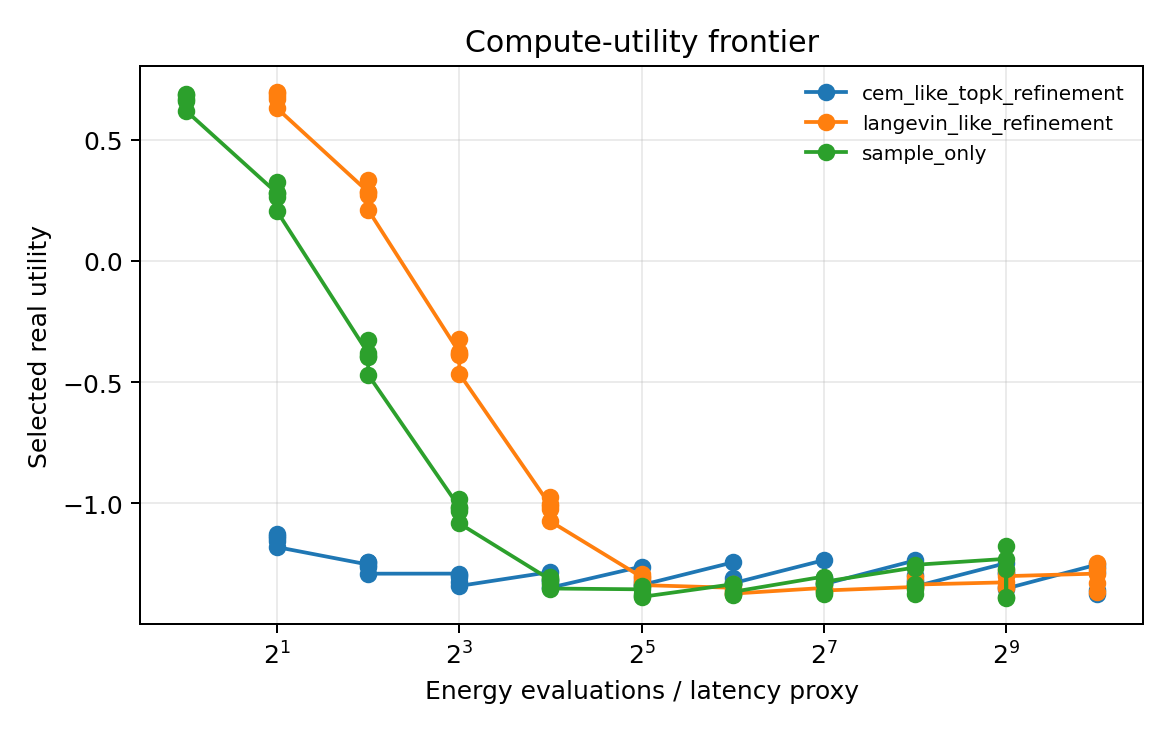
\includegraphics[width=\linewidth]{figure5_compute_utility_frontier.png}
    \end{minipage}
    \caption{Selected-tail reliability and compute frontier. The diagnostics ask whether the low-energy tail is useful, not merely whether average score statistics look reasonable.}
    \label{fig:reliability-compute}
\end{figure}

\subsection{Simulator evidence is artifact-scoped}

Table~\ref{tab:metaworld-selected} reports the selected-action Meta-World ladder. The primary expert-action-trained EBM reaches success \(1.0\) on all four tasks under the selected-action plus scripted-continuation evaluation. Calibrated scoring improves selected reward on the same artifacts. This supports finite simulator benchmark execution, not autonomous long-horizon learned-policy success.

\begin{table}[t]
\centering
\small
\setlength{\tabcolsep}{4pt}
\begin{tabular}{lrrrr}
\toprule
Task & Expert EBM reward & Calibrated reward & Success & Max law error \\
\midrule
button-press-v3 & 0.893 & 0.909 & 1.0 & 0.0003 \\
pick-place-v3 & 5.331 & 5.567 & 1.0 & 0.0016 \\
push-v3 & 5.726 & 6.215 & 1.0 & 0.0022 \\
reach-v3 & 8.326 & 8.581 & 1.0 & 0.0198 \\
\bottomrule
\end{tabular}
\caption{Meta-World selected-action benchmark. The selected first action is followed by scripted continuation; therefore this table is not autonomous learned-policy evidence.}
\label{tab:metaworld-selected}
\end{table}

The closed-loop dependency audit in Table~\ref{tab:closed-loop} removes scripted continuation and averages over tasks. Expert-centered candidates with a gate succeed but depend on runtime expert-centered proposals. State-heuristic variants clear the low-dependency threshold, including the EBM-selected state-heuristic proposal variant. The learned nearest-demo, behavior-cloned, and local Gaussian variants do not clear the learned-policy threshold across tasks. Thus the supported claim is a dependency audit: state-heuristic low-dependency variants clear the threshold, while autonomous learned-policy Meta-World success remains unsupported.

\begin{table}[t]
\centering
\small
\setlength{\tabcolsep}{3pt}
\begin{tabular}{p{0.42\linewidth}rrr}
\toprule
Closed-loop policy & Success & Reward & Fallback \\
\midrule
expert-centered gate & 1.00 & 145.10 & 0.143 \\
expert-centered no gate & 0.65 & 117.22 & 0.000 \\
learned-demo proposal + EBM & 0.30 & 166.52 & 0.000 \\
behavior-cloned proposal + EBM & 0.40 & 138.34 & 0.000 \\
local Gaussian + EBM & 0.05 & 117.98 & 0.000 \\
state heuristic proposal + EBM & 1.00 & 143.28 & 0.000 \\
state heuristic direct & 1.00 & 143.14 & 0.000 \\
random uniform & 0.00 & 55.40 & 0.000 \\
scripted expert & 1.00 & 143.14 & 0.000 \\
\bottomrule
\end{tabular}
\caption{Closed-loop Meta-World dependency audit without scripted continuation, averaged across the four tasks. Learned-policy variants do not clear the threshold; state-heuristic variants do.}
\label{tab:closed-loop}
\end{table}

\begin{figure}[t]
    \centering
    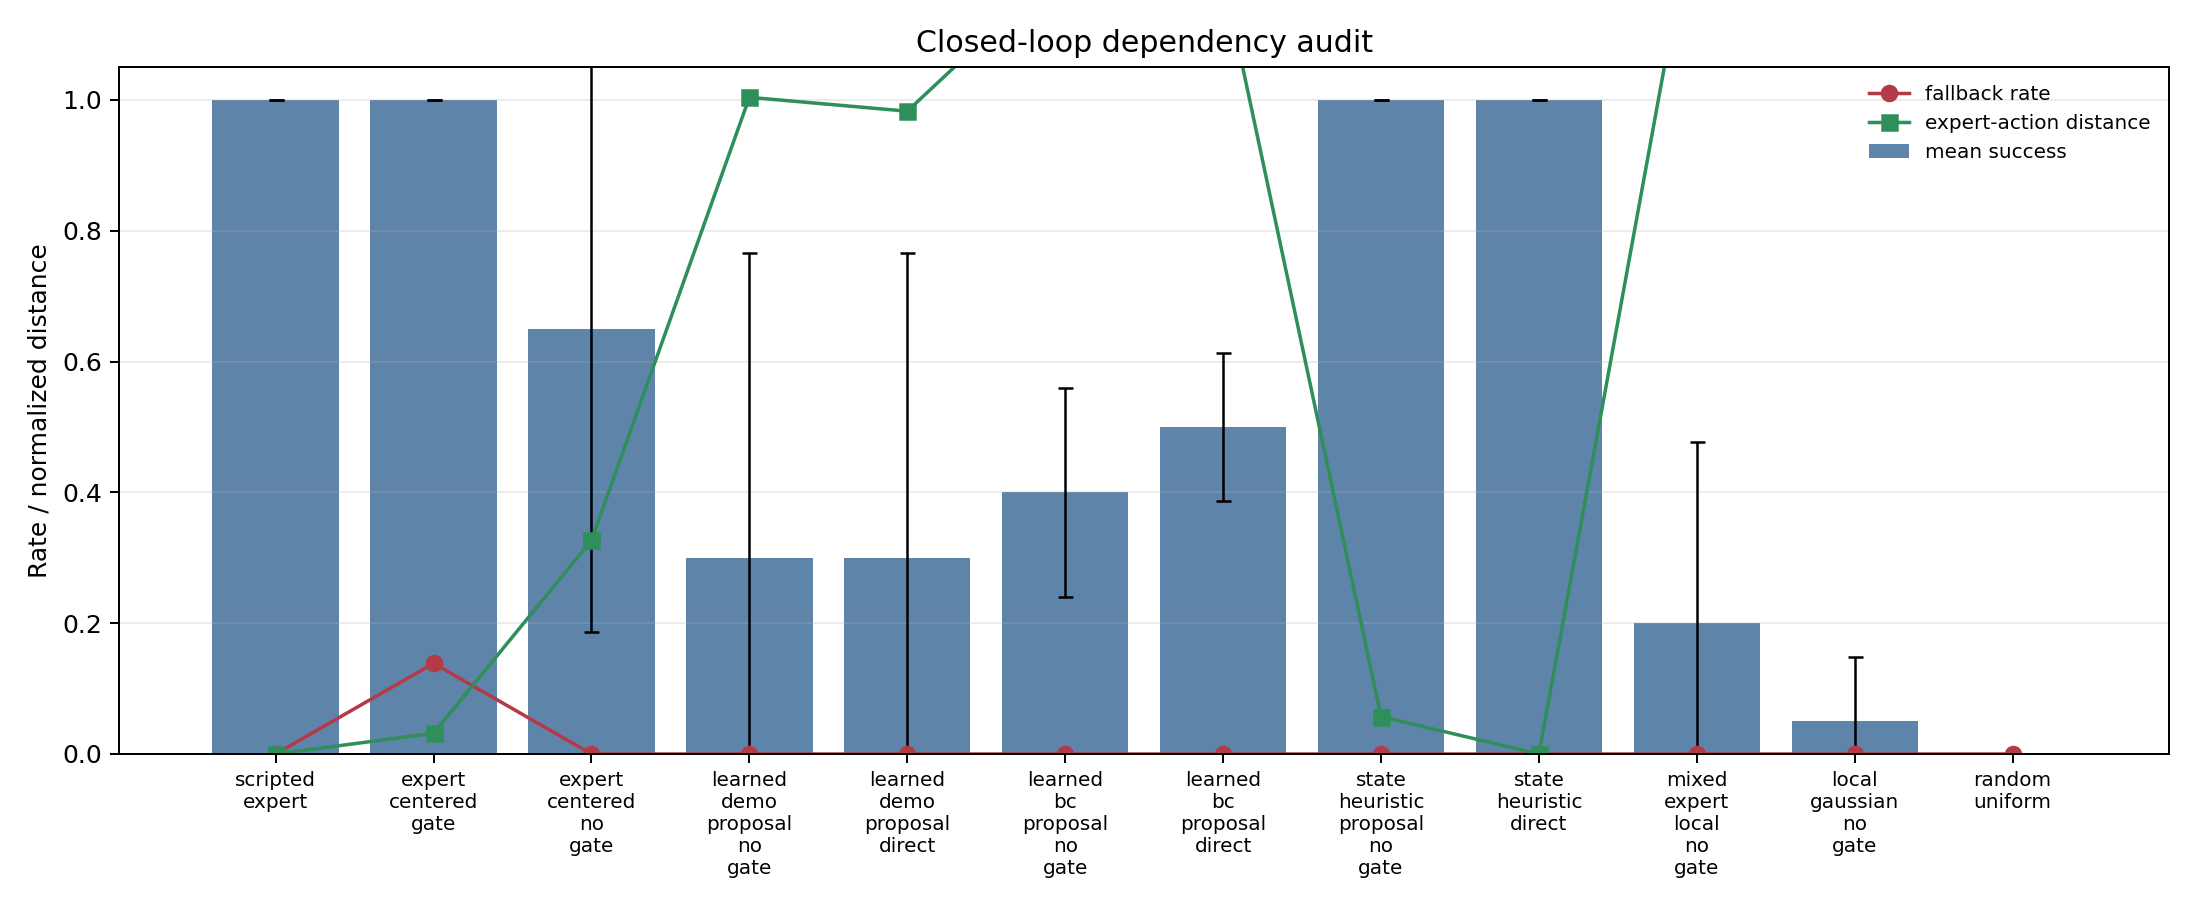
\includegraphics[width=0.95\linewidth]{figure10_closed_loop_dependency_audit.png}
    \caption{Closed-loop dependency audit. The figure separates expert-centered, learned-proposal, state-heuristic, random, and scripted variants so the supported claim does not overstate autonomy.}
    \label{fig:dependency}
\end{figure}

\section{Related Work}

Energy-based learning frames prediction as assigning low energy to compatible configurations and high energy otherwise \citep{lecun2006tutorial,du2019implicit}. Implicit Behavioral Cloning applies this idea to action selection by learning an energy over observation-action pairs and optimizing actions at inference time \citep{florence2022implicit}. Diffusion policies and other sampling-based robot policies also expose inference-time candidate or refinement budgets, although their failure modes need not be identical to EBM low-energy-tail miscalibration \citep{chi2023diffusionpolicy}. Our finite law is closest in spirit to order-statistic analyses \citep{david2003order}, but the emphasis here is the utility of the selected score tail under a fixed robot-policy stack. Calibration and reliability diagrams are standard tools for neural prediction \citep{guo2017calibration}; we adapt the question to selected energy quantiles and real utility.

\section{Limitations and Scope}

The theorem is conditional on a fixed candidate generator, scorer, and utility measurement. It does not prove a universal EBM guarantee, a universal benefit from tail selection, or a universal calibration repair. The strongest failures are controlled or small learned-policy artifacts designed to isolate the selected-tail mechanism. The Meta-World selected-action ladder uses scripted continuation after the selected action. The closed-loop audit removes scripted continuation, but the current learned nearest-demo, behavior-cloned, and local variants leave autonomous learned-policy success unsupported. Optional Gymnasium, ManiSkill, and robosuite rollouts are finite guarded adapter checks. No real-robot validation is claimed.

\section{Reproducibility}

All promoted claims are tied to local CSV/JSON artifacts and regenerated figures. The exact-law validation, claim audit, and tests are part of the artifact workflow. An anonymized artifact will be provided as supplementary material, including scripts to rebuild the figures and this anonymous PDF.

\section{Conclusion}

tail selection inference for EBMs is selected low-energy-tail optimization. The finite law predicts selected utility for any fixed stack, and the experiments show why the law matters: energy can improve while utility degrades when the low-energy tail is miscalibrated. Reliability diagrams, support diagnostics, pilot-label calibration, and conservative gates provide a practical audit and repair framework, but their claims must remain tied to the measured tail and the artifact scope.

\bibliographystyle{iclr2026_conference}
\bibliography{refs}

\appendix
\section{Appendix}

\subsection{Finite-law derivation}

For completeness, we derive Equation~\ref{eq:finite-law}. Let \(G_k\) be the \(k\)-th score group in descending score order and let \(C_k\) be the cumulative proposal mass of groups \(1,\ldots,k\). The event that group \(k\) is selected is the event that no sample lands in groups \(1,\ldots,k-1\) and at least one sample lands in group \(k\). Its probability is
\[
    \Pr(\mathrm{sel}=G_k) =
    (1-C_{k-1})^N - (1-C_k)^N .
\]
Conditional on this event, all selected candidates have score \(s_k\). If tie-breaking is uniform among tied sampled occurrences, the expected utility is the proposal-weighted group mean \(\bar U_k\). Summing over groups gives the exact finite selected-utility law.

\subsection{Artifact map}

\begin{table}[h]
\centering
\small
\setlength{\tabcolsep}{4pt}
\begin{tabular}{p{0.33\linewidth}p{0.58\linewidth}}
\toprule
Claim area & Local artifacts \\
\midrule
Exact finite law & \texttt{results/exact\_law/summary.json}, \texttt{validation.csv} \\
Controlled low-energy tail failure & \texttt{results/controlled\_energy\_tail/summary.json}, \texttt{seed\_level.csv} \\
Learned IBC-style EBMs & \texttt{results/learned\_ibc/summary.json}, \texttt{results/learned\_torch\_ibc/summary.json} \\
Repair hierarchy & \texttt{results/repair/summary.json}, \texttt{results/repair\_effectiveness/summary.json} \\
Reliability diagrams & \texttt{results/reliability/summary.csv}, \texttt{figure3\_tail\_reliability.png} \\
Meta-World benchmark ladder & \texttt{results/benchmarks/metaworld/task\_table.csv} \\
Closed-loop dependency audit & \texttt{closed\_loop\_ablation\_summary.csv}, \texttt{closed\_loop\_ablation\_policy\_summary.csv} \\
Optional adapters & \texttt{results/optional\_benchmarks/summary.json}, \texttt{rollouts.csv} \\
Claim audit & \texttt{results/claims\_status.json}, \texttt{docs/claims.md} \\
\bottomrule
\end{tabular}
\caption{Artifact paths used by the paper. Paths are relative to the repository root.}
\label{tab:artifact-map}
\end{table}

\subsection{Claim ledger summary}

\begin{table}[h]
\centering
\small
\setlength{\tabcolsep}{4pt}
\begin{tabular}{p{0.27\linewidth}p{0.62\linewidth}}
\toprule
Status & Paper claim boundary \\
\midrule
Supported & Finite tie-aware law predicts selected utility for a fixed score/utility pool. \\
Supported & Controlled and learned IBC-style EBMs can over-optimize a miscalibrated low-energy tail. \\
Supported & Reliability buckets expose the extreme low-energy tail and report utility, success, support, and contact diagnostics. \\
Supported & The main repair stack nearly closes the measured high-\(N\) gap by the predefined recovery ratio. \\
Supported & Meta-World selected-action artifacts use scripted expert actions as primary positives and scripted continuation for rollout reward. \\
Supported & State-heuristic no-gate Meta-World variants clear the low-dependency threshold in the closed-loop audit. \\
Unsupported non-claim & No real-robot validation is present. \\
Unsupported non-claim & Autonomous learned-policy Meta-World success remains unsupported. \\
Unsupported non-claim & Broad manipulation success is not claimed. \\
\bottomrule
\end{tabular}
\caption{Condensed claim ledger. The full ledger is in \texttt{docs/claims.md} and \texttt{results/claims\_status.json}.}
\label{tab:claim-ledger}
\end{table}

\subsection{Repair stress details}

\begin{table}[h]
\centering
\small
\setlength{\tabcolsep}{4pt}
\begin{tabular}{lrrrr}
\toprule
Repair model at \(N=512\) & Mean recovery & Worst recovery & Failures & Utility-degrading \\
\midrule
support penalized & 0.886 & 0.836 & 5 & 0 \\
support penalized + gate & 0.870 & 0.735 & 5 & 0 \\
value shaped & 0.904 & 0.892 & 5 & 0 \\
calibrated & 0.972 & 0.960 & 1 & 0 \\
calibrated + support + gate & 0.972 & 0.962 & 1 & 0 \\
oracle & 1.000 & 1.000 & 0 & 0 \\
\bottomrule
\end{tabular}
\caption{Repair stress matrix summary. Failures count configured diagnostic failures, not hidden utility regressions.}
\label{tab:repair-stress}
\end{table}

\subsection{Optional guarded rollout adapters}

\begin{table}[h]
\centering
\small
\setlength{\tabcolsep}{4pt}
\begin{tabular}{llrrr}
\toprule
Suite & Task & Seeds & Mean reward & Success \\
\midrule
Gymnasium & Pusher-v5 & 2 & -18.417 & n/a \\
ManiSkill & PickCube-v1 & 2 & 0.987 & 0.000 \\
ManiSkill & PushCube-v1 & 2 & 1.297 & 0.000 \\
robosuite & Door & 2 & 0.034 & 0.000 \\
robosuite & Lift & 2 & 55.757 & 0.275 \\
\bottomrule
\end{tabular}
\caption{Optional non-Meta-World adapters. These are finite guarded rollout artifacts only.}
\label{tab:optional}
\end{table}

\subsection{Additional figures}

\begin{figure}[h]
    \centering
    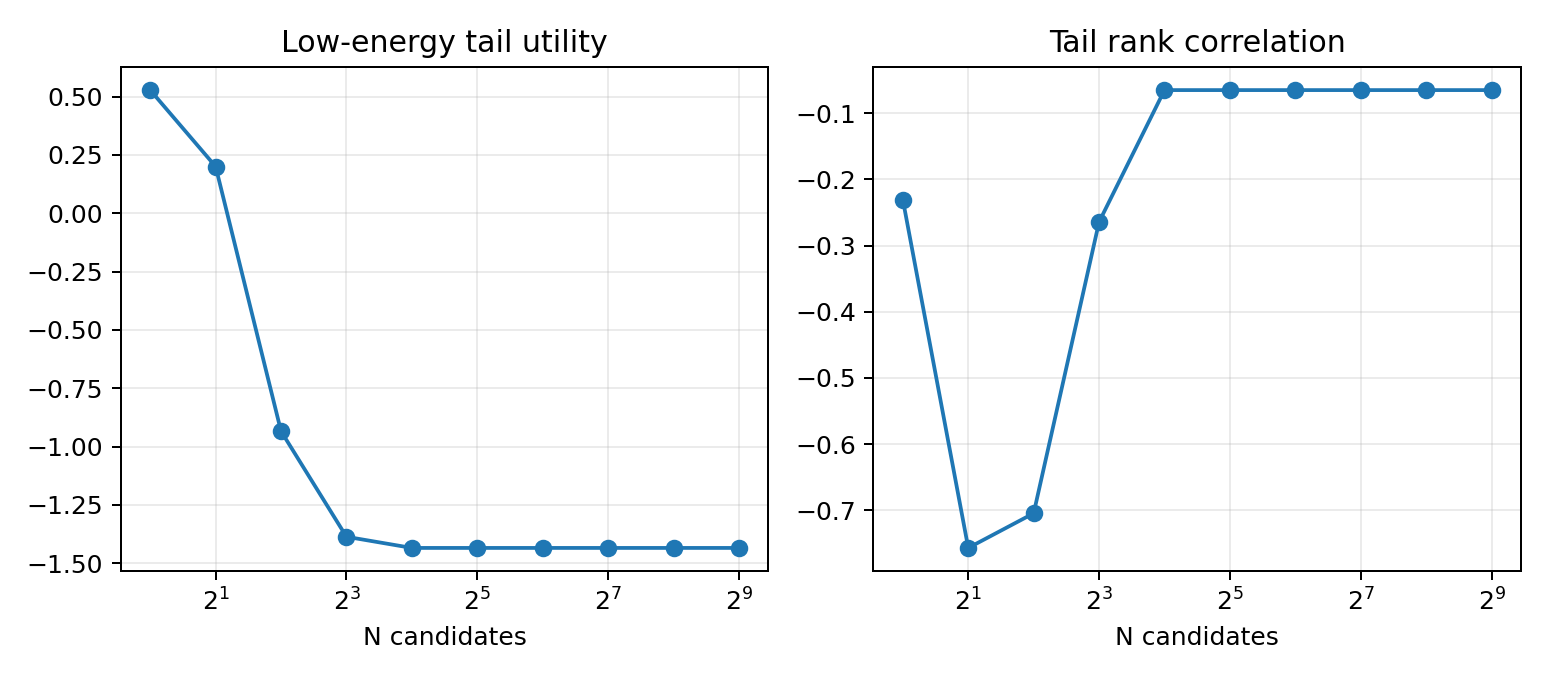
\includegraphics[width=0.95\linewidth]{figure4_tail_rank_and_tail_utility.png}
    \caption{Tail rank and tail utility diagnostics.}
    \label{fig:tail-rank-appendix}
\end{figure}

\begin{figure}[h]
    \centering
    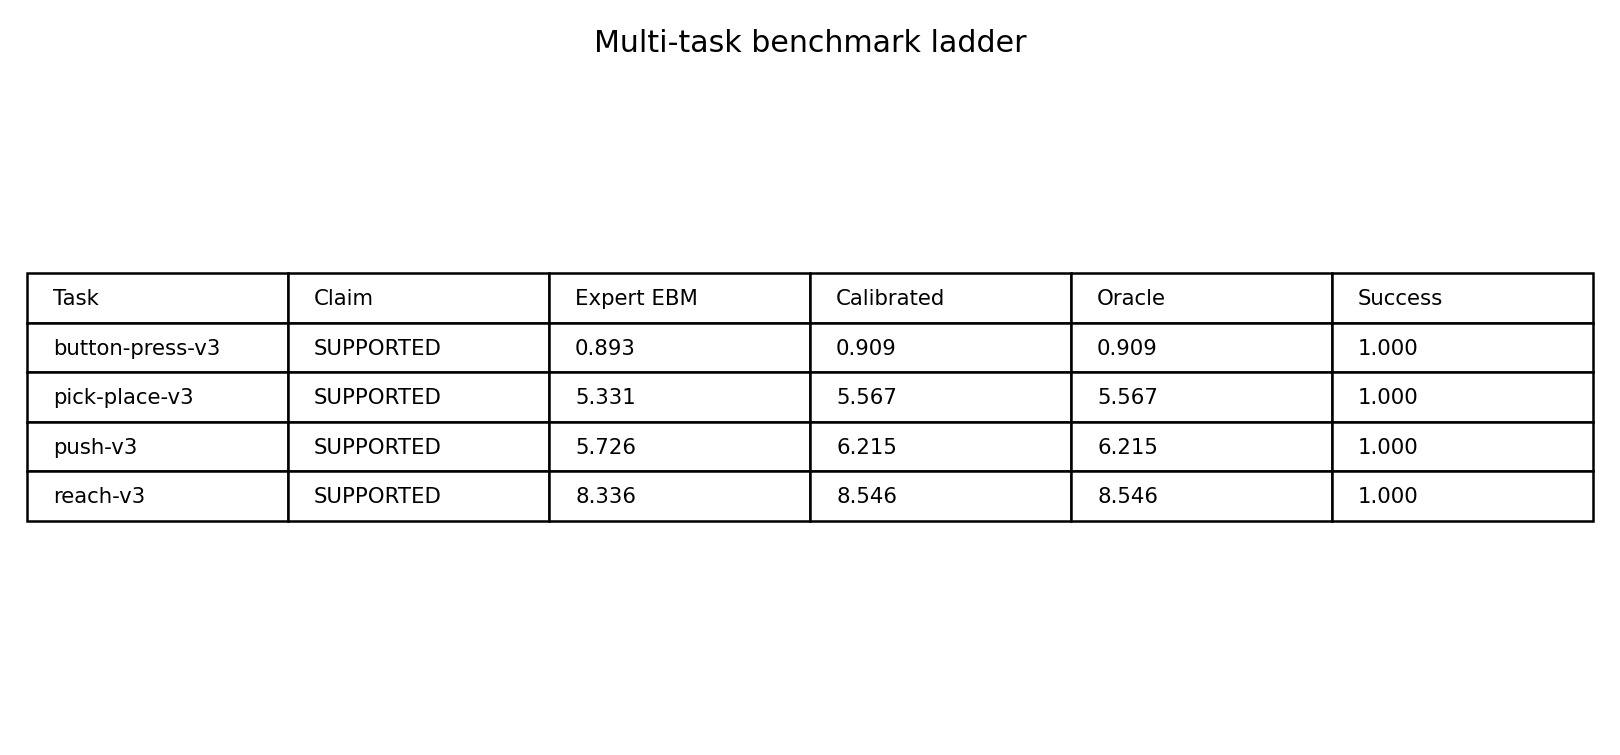
\includegraphics[width=0.95\linewidth]{figure6_multitask_benchmark_table.png}
    \caption{Generated multi-task benchmark table.}
    \label{fig:benchmark-table-appendix}
\end{figure}

\begin{figure}[h]
    \centering
    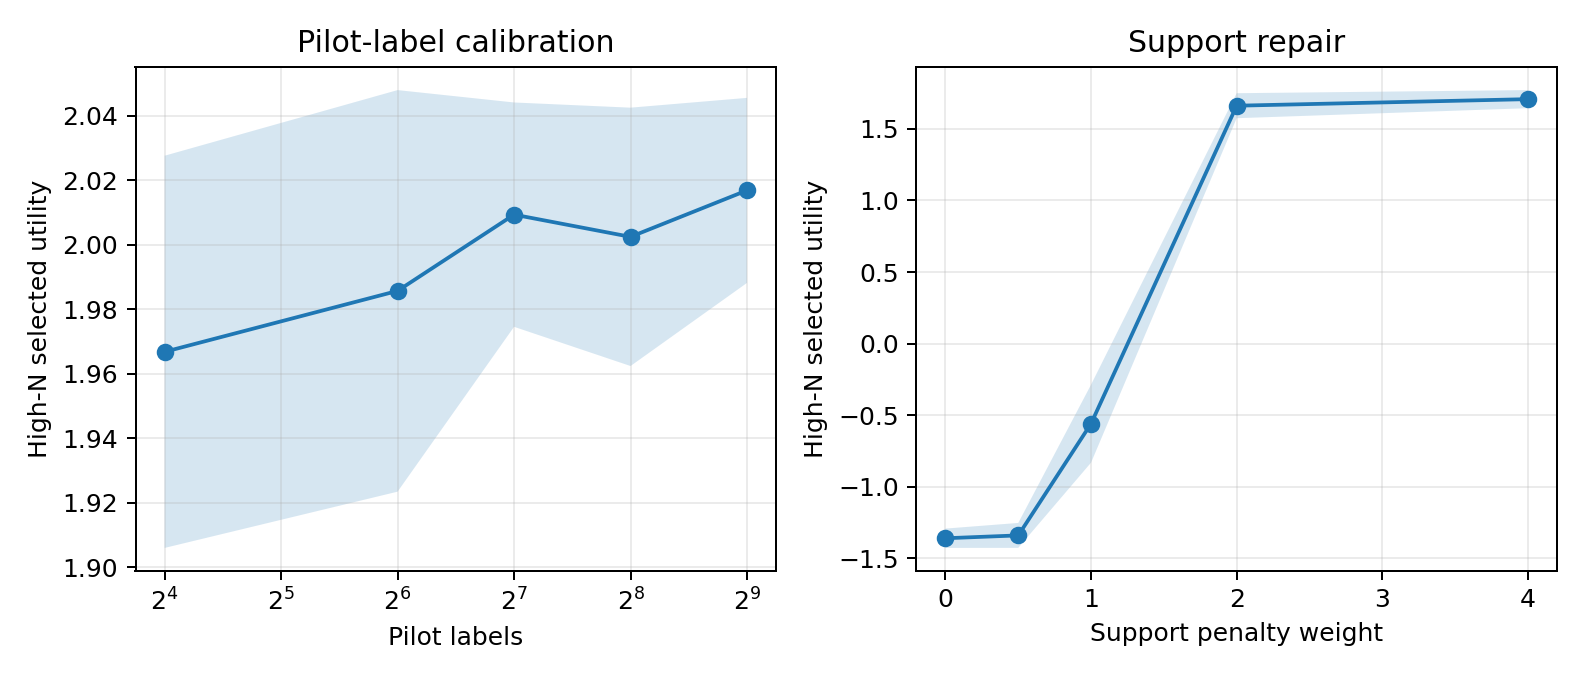
\includegraphics[width=0.95\linewidth]{figure7_repair_ablations.png}
    \caption{Repair ablations.}
    \label{fig:repair-ablations-appendix}
\end{figure}

\begin{figure}[h]
    \centering
    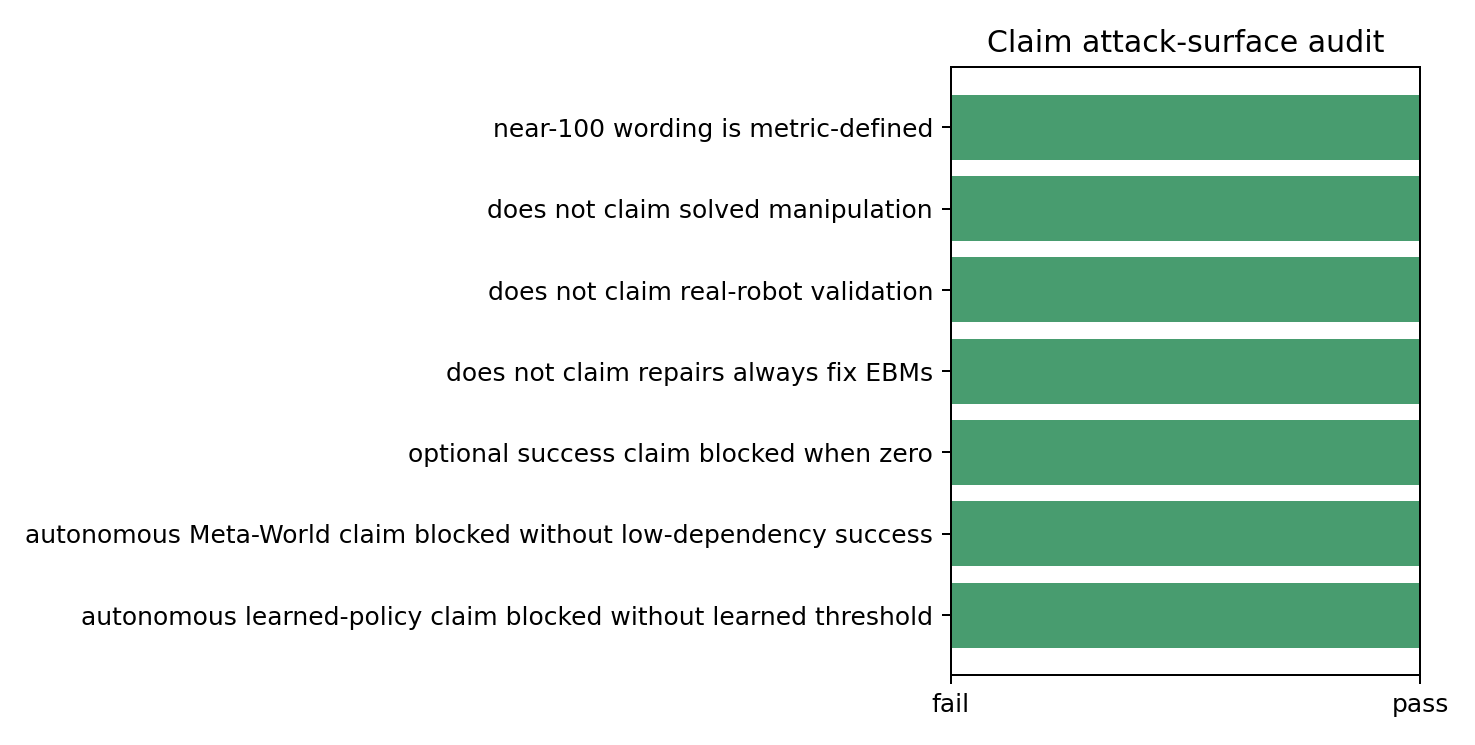
\includegraphics[width=0.95\linewidth]{figure9_attack_surface_audit.png}
    \caption{Attack-surface and claim-boundary audit figure.}
    \label{fig:attack-surface-appendix}
\end{figure}

\subsection{Reproducibility commands}

The anonymous paper PDF can be rebuilt from the repository root with:
\begin{center}
\small
\texttt{powershell -ExecutionPolicy Bypass -File}\\
\texttt{scripts/build\_iclr\_paper.ps1}
\end{center}
The claim audit can be run with \texttt{bash scripts/run\_claim\_audit.sh}. The test suite can be run with \texttt{pytest}. Long simulator refreshes are intentionally not required for rebuilding the paper because the paper consumes the existing CSV/JSON/PNG artifacts.


\end{document}
